%% The first command in your LaTeX source must be the \documentclass command.
%%
%% Options:
%% twocolumn : Two column layout.
%% hf: enable header and footer.
\documentclass[
% twocolumn,
% hf,
]{ceurart}

%%
%% One can fix some overfulls
\sloppy

%%
%% Minted listings support 
%% Need pygment <http://pygments.org/> <http://pypi.python.org/pypi/Pygments>
\usepackage{listings}
\usepackage{amsmath, amssymb, amsfonts}
\usepackage{float, graphicx, color, xcolor, colortbl}
%% auto break lines
\lstset{breaklines=true}

%%
%% end of the preamble, start of the body of the document source.
\begin{document}

% %%
% %% Rights management information.
% %% CC-BY is default license.
\copyrightyear{2022}
\copyrightclause{Copyright for this paper by its authors.
  Use permitted under Creative Commons License Attribution 4.0
  International (CC BY 4.0).}

%%
%% This command is for the conference information
\conference{}

%%
%% The "title" command
\title{CLEF 2025 PAN: Multi-Author Writing Style Analysis}

% \tnotemark[1]
% \tnotetext[1]{You can use this document as the template for preparing your
%   publication. We recommend using the latest version of the ceurart style.}

%%
%% The "author" command and its associated commands are used to define
%% the authors and their affiliations.
\author[1]{Ali Muhammad Asad}[email=aa07190@st.habib.edu.pk]
\address[1]{Department of Computer Science, Habib University}

\author[2]{Musaib}[email=mu07694@st.habib.edu.pk]
\address[2]{Department of Computer Science, Habib University}

\author[3]{Syed Muhammad Areeb Kazmi}[email=mk07202@st.habib.edu.pk]
\address[3]{Department of Computer Science, Habib University}

\author[4]{Sarim Tahir}[email=st07112@st.habib.edu.pk]
\address[4]{Department of Computer Science, Habib University}

% %% Footnotes
% \cortext[1]{Corresponding author.}
% \fntext[1]{These authors contributed equally.}

%%
%% The abstract is a short summary of the work to be presented in the
%% article.
\begin{abstract}
    Multi-Author Writing Style Analysis is a crucial task in computational linguistics and authorship attribution, aimed at identifying points of transition within a document. This task has significant applications in forensic linguistics, plagiarism detection, and content verification. Over the years, various approaches have been explored, ranging from traditional stylometric techniques to advanced deep learning models. Early research relied on lexical and syntactic features to detect style changes, but these methods faced limitations in handling nuanced transitions. Recent advancements, particularly the integration of transformer-based models, have significantly improved the accuracy of style change detection. This paper aims to provide an overview of the tasks, the datasets, the evaluation metrics, and the baseline models for the Multi-Author Writing Style Analysis Lab of the PAN track at CLEF 2025.
\end{abstract}

% %%
% %% Keywords. The author(s) should pick words that accurately describe
% %% the work being presented. Separate the keywords with commas.
% \begin{keywords}
%   LaTeX class \sep
%   paper template \sep
%   paper formatting \sep
%   CEUR-WS
% \end{keywords}

%%
%% This command processes the author and affiliation and title
%% information and builds the first part of the formatted document.
\maketitle

\section{Introduction}

Writing style analysis is a fundamental problem in computational linguistics, with applications in authorship attribution, forensic text analysis, and collaborative content verification. A challenge in this domain is detecting when authorship changes within a multi-author document, a task known as style change detection. This problem has been the focus of multiple iterations of the PAN shared tasks, which have provided benchmark datasets and evaluation frameworks to advance the field.

Early approaches to style change detection leveraged handcrafted features such as n-grams, part-of-speech tag frequencies, and sentence structure analysis. These methods, while effective for basic segmentation tasks, struggled with complex, subtle changes in authorial style. The introduction of deep learning and pre-trained transformer models revolutionized the field, allowing for more nuanced analysis of writing styles. Models like BERT and DeBERTa have demonstrated superior performance in detecting stylistic shifts at both the paragraph and sentence levels.

This paper aims to explore existing methods and challenges in multi-author writing style analysis, reviewing state-of-the-art approaches such as deep learning models, transfer learning, and ensemble techniques. We will discuss the datasets, evaluation metrics, and baseline models used in the previous iterations of Multi-Author Writing Style Analysis Lab of the PAN track, ultimately attempting to improve the performance of style change detection.

\section{Literature Review}

Traditional approaches to multi-author writing style analysis have relied on lexical and syntactic feature-based methods, including TF-IDF vectorization, character n-grams, and POS tag frequencies. These techniques have demonstrated moderate performance in detecting style changes at the paragraph level but struggle with sentence-level changes due to limited contextual understanding. One study leveraged a combination of lexical and structural features, such as indentation and sentence length, to refine style change detection by incorporating discourse-level analysis. However, handcrafted features were constrained by their susceptibility to topic influence, leading to inconsistent performance across datasets \cite{paper6} \cite{paper4}.

More recent approaches of 2024 and 2023 have shifted towards deep learning and transformer-based models to address these limitations. A paper in PAN 2024 explored bagging techniques, feature engineering, BERT-based classifiers and ensemble techniques combining different architectures such as BERT, RoBERTa, Electra and Llama2, using DetectGPT (Mistral-7B Falcon-7B) as their baseline models. They were able to achieve an F1-score of 0.924 as their best results on fine-tuned Mistral and Llama2 models \cite{paper1}. Another noteworthy paper of 2023 leveraged pre-trained transformers like DeBERTaV3 and BERT for paragraph-level classification, achieving state-of-the-art F1 scores of 0.83 for the hardest dataset variant \cite{paper3}. These models incorporated contrastive learning and fine-tuning on task-specific datasets, allowing them to distinguish between subtle stylistic variations more effectively. However, their performance degraded when topic variations were minimized, highlighting the challenge of isolating style from content. 

Another approach was used in 2023 where the authors performed data augmentation before training several models including RoBERTa, ELECTRA, and BERT. They achieved the best scores on RoBERTa with F1 scores of 0.996, 0.811, 0.814 for easy, medium, and hard datasets respectively \cite{paper_2023_1}. Another paper decided to use a different approach where they used a contrastive learning method to optimize the segment embedding output by the encoder of the pre-training model to obtain more similar vector spaces when processing sentences with similar styles. They called this CoSENT, and were able to get F1 scores of 0.915, 0.820, and 0.705 on easy, medium, and hard datasets respectively \cite{paper_2023_2}.

Tzu-Mi Lin et.al experimented with ensemble pre-trained transformer models including BERT, RoBERTa, and ALBERT. The best scores they got were for RoBERTa overall with F1 scores of 0.766, 0.503, and 0.705 for easy, medium, and hard datasets respectively \cite{paper_2022}. Hybrid Deep learning models have also been explored such as Bi-LSTM and BERT where BERT was used to create word embeddings which were then passed onto a BI-LSTM layer, followed by a CNN layer, then by a pooling layer, and finally through a fully connected layer \cite{paper_2022_2}. This model achieved F1 scores of 0.67, 0.40, and 0.65 for easy, medium, and hard datasets respectively.

% Traditional approaches to multi-author writing style analysis mainly rely on lexical and syntactic feature based methods such as TF-IDF vectorization, character n-grams, and POS tag frequencies. These methods have demonstrated moderate performance in detecting style change at the paragraph level, but struggle with sentence-level changes due to limited contextual understanding. For instance, the PAN 2021 task utilized lexical similarity measures to detect authorship changes, achieving an F1 score of 0.73 on multi-author documents, indicating that feature-based methods were more effective for document-wide analysis but struggled with fine-grained author attribution \cite{paper6}. PAN 2022 introduced structural features such as indentation and average sentence length, further refining style change detection by incorporating discourse-level analysis \cite{paper4}. However, these methods were constrained by their reliance on handcrafted features and were susceptible to topic influence.

% PAN 2023 and 2024 introduced more powerful techniques such as transformer based methods. The top-performing models in PAN 2023 leveraged pre-trained transformers like DeBERTaV3 and BERT for paragraph-level classification, achieving state-of-the-art F1 scores of 0.83 for the hardest dataset variant \cite{paper3}. These models incorporated contrastive learning and fine-tuning on task-specific datasets, allowing them to distinguish between subtle stylistic variations more effectively. However, their performance degraded when topic variations were minimized, highlighting the challenge of isolating style from content.

% Another approach integrated contrastive learning with DeBERTaV3 and knowledge distillation for efficiency \cite{paper3}. This method allowed models to refine their representations of stylistic shifts while maintaining computational feasibility. Additionally, multi-stage fine-tuning techniques were introduced in PAN 2024, further improving performance by integrating both syntactic and semantic embeddings for style differentiation \cite{paper2}. Hybrid approaches were also explored, combining traditional and deep learning methods. One study used a stacking ensemble of lexical and neural models, achieving an F1 score of 0.82 on medium-difficulty datasets \cite{paper3}. Another team experimented with sentence-level style change detection using hierarchical clustering and transformer embeddings, demonstrating the potential for finer granularity in authorship attribution \cite{paper2}.

% Performance evaluation has been standardized using the macro-averaged F1-score, with separate rankings for easy, medium, and hard datasets. PAN 2023 results highlighted the superiority of transformer-based models over traditional techniques, with the best-performing systems leveraging multi-stage fine-tuning, semantic similarity post-processing, and ensemble classifiers \cite{paper2}. However, performance variations across dataset difficulty levels suggest that improvements in data augmentation and domain adaptation are needed. Another paper in PAN 2024 explored bagging techniques, feature engineering, BERT-based classifiers and ensemble techniques combining different architectures such as BERT, RoBERTa, Electra and Llama2, using DetectGPT (Mistral-7B Falcon-7B) as their baseline models. They were able to achieve an F1-score of 0.924 as their best results on fine-tuned Mistral and Llama2 models \cite{paper1}.


\section{Methodology}
\subsection{Dataset}
The dataset was provided by PAN, based on user posts from various subreddits of the Reddit platform. It is divided into three levels: easy, medium and hard, where each level is split into three parts:
\begin{itemize}
    \item \textit{training set:} Contains 70\% of the whole dataset and includes ground truth data. This data would be used to develop and train the models.
    \item \textit{validation set:} Contains 15\% of the whole dataset and includes ground truth data. This data would be used to evaluate and optimize the models.
    \item \textit{test set:} Contains 15\% of the whole dataset and does not include ground truth data. This data would be used to evaluate the models.
\end{itemize}

\subsubsection*{Input Format}
For each problem instance X (i.e., each input document), two files are provided:
\begin{enumerate}
    \item \textit{problem-X.txt} which contains the actual text in the form of sentences of varying lengths.
    \item \textit{truth-problem-X.json} which contains the ground truth, i.e., the correct solution in JSON format. 
\end{enumerate}

\noindent A sample json file looks as so:
\begin{verbatim}
{"authors": 2,
"changes": [0, 0, 0, 0, 0, 0, 0, 0, 1, 0, 0, 0]}
\end{verbatim}
where the key `changes' is an array of consecutive sentences within each document (0 when there is no change, and 1 when there is a change). 

\subsection{Initial Approach}
The initial approach, which is also our baseline, was to use the Bag of Words (BoW) method for feature extraction from the sentences, coupled with a simple logistic regression model for classification. The Bag of Words method is a simple and effective way to represent text data. It involves creating a vocabulary of unique words and then representing each sentence as a vector of word counts. This became our baseline approach, as it is simple and easy to implement, and was backed by previous implementations \cite{paper1}.

Once our baseline was set, we modified the bag of words approach to combine n-grams and syntactic/lexical features (sentence length, POS tag frequencies, etc), along with calss weighting to handle the class imbalance between instances of 0s and 1s, and finally used a vectorized tuning with ngram\_range of (1, 2) to include both unigrams and bigrams in the feature set, in order to improve the model's performance by capturing more context and semantics from the text data. This showed an improvement in the model's performance over the baseline. 

\section{Results}

This section presents the results of our experiments. The table below shows the performance of the models on the validation set. The models were evaluated based on the F1 score, which is the harmonic mean of precision and recall. The F1 score is a good metric for imbalanced datasets, as it considers both false positives and false negatives. The F1 score is presented for each level, easy, medium and hard.

\begin{table}[ht]
\centering
\begin{tabular}{|l|l|l|l|}
    \hline
    \textbf{Level} & \textbf{F1 (Easy)} & \textbf{F1 (Medium)} & \textbf{F1 (Hard)} \\ \hline
    \textbf{Baseline BoW} & 0.65 & 0.65 & 0.57 \\ \hline
    \textbf{Improved BoW} & 0.79 & 0.67 & 0.61 \\ \hline
\end{tabular}
\caption{F1 scores of the models on the validation set}
\end{table}

The results show an improvement in the F1 score for the improved BoW model over the baseline BoW model on all levels. 

% \subsection{Title Information}

% The titles of papers should be either all use the emphasizing
% capitalized style or they should all use the regular English (or
% native language) style. It does not make a good impression if you or
% your authors mix the styles.

% Use the \verb|\title| command to define the title of your work. Do not
% insert line breaks in your title.

% \subsection{Authors and Affiliations}

% Each author must be defined separately for accurate metadata
% identification. Multiple authors may share one affiliation. Authors'
% names should not be abbreviated; use full first names wherever
% possible. Include authors' e-mail addresses whenever possible.

% \verb|\author| command have the below options: 

% \begin{itemize}
% \item \verb|style| : Style of author name (chinese)
% \item \verb|prefix| : Prefix
% \item \verb|suffix| : Suffix
% \item \verb|degree| : Degree
% \item \verb|role| : Role
% \item \verb|orcid| : ORCID
% \item \verb|email| : E-mail
% \item \verb|url| : URL
% \end{itemize}

% Author names can have some kinds of marks and notes:
% \begin{itemize}
% \item affiliation mark: \verb|\author[<num>]|.
% \end{itemize}

% The author names and affiliations could be formatted in two ways:
% \begin{enumerate}
% \item Group the authors per affiliation.
% \item Use an explicit mark to indicate the affiliations.
% \end{enumerate}

% Author block example:
% \begin{lstlisting}
% \author[1,2]{Author Name}[%
%     prefix=Prof.,
%     degree=D.Sc.,
%     role=Researcher,
%     orcid=0000-0000-000-0000,
%     email=name@example.com,
%     url=https://name.example.com
% ]

% \address[1]{Affiliation #1}
% \address[2]{Affiliation #2}
% \end{lstlisting}

% \subsection{Abstract and Keywords}

% Abstract shall be entered in an environment that starts
% with \verb|\begin{abstract}| and ends with
% \verb|\end{abstract}|. 

% \begin{lstlisting}
% \begin{abstract}
%   This is an abstract.
% \end{abstract}
% \end{lstlisting}



% \section{Tables}

% The ``\verb|ceurart|'' document class includes the ``\verb|booktabs|''
% package --- \url{https://ctan.org/pkg/booktabs} --- for preparing
% high-quality tables.

% Table captions are placed \textit{above} the table.

% Because tables cannot be split across pages, the best placement for
% them is typically the top of the page nearest their initial cite.  To
% ensure this proper ``floating'' placement of tables, use the
% environment \verb|table| to enclose the table's contents and the
% table caption. The contents of the table itself must go in the
% \verb|tabular| environment, to be aligned properly in rows and
% columns, with the desired horizontal and vertical rules.

% Immediately following this sentence is the point at which
% Table~\ref{tab:freq} is included in the input file; compare the
% placement of the table here with the table in the printed output of
% this document.

% \begin{table*}
%   \caption{Frequency of Special Characters}
%   \label{tab:freq}
%   \begin{tabular}{ccl}
%     \toprule
%     Non-English or Math&Frequency&Comments\\
%     \midrule
%     \O & 1 in 1,000& For Swedish names\\
%     $\pi$ & 1 in 5& Common in math\\
%     \$ & 4 in 5 & Used in business\\
%     $\Psi^2_1$ & 1 in 40,000& Unexplained usage\\
%   \bottomrule
% \end{tabular}
% \end{table*}

% To set a wider table, which takes up the whole width of the page's
% live area, use the environment \verb|table*| to enclose the table's
% contents and the table caption.  As with a single-column table, this
% wide table will ``float'' to a location deemed more
% desirable. Immediately following this sentence is the point at which
% Table~\ref{tab:commands} is included in the input file; again, it is
% instructive to compare the placement of the table here with the table
% in the printed output of this document.

% \begin{table}
%   \caption{Some Typical Commands}
%   \label{tab:commands}
%   \begin{tabular}{ccl}
%     \toprule
%     Command &A Number & Comments\\
%     \midrule
%     \texttt{{\char'134}author} & 100& Author \\
%     \texttt{{\char'134}table}& 300 & For tables\\
%     \texttt{{\char'134}table*}& 400& For wider tables\\
%     \bottomrule
%   \end{tabular}
% \end{table}


% \section{Figures}

% The ``\verb|figure|'' environment should be used for figures. One or
% more images can be placed within a figure. If your figure contains
% third-party material, you must clearly identify it as such, as shown
% in the example below.
% \begin{figure}
%   \centering
%   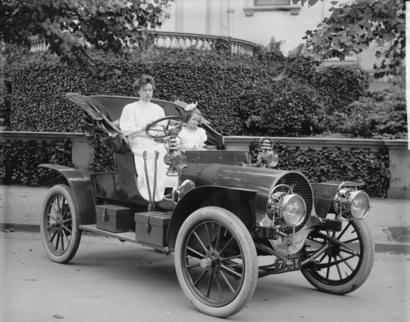
\includegraphics[width=\linewidth]{sample-franklin}
%   \caption{1907 Franklin Model D roadster. Photograph by Harris \&
%     Ewing, Inc. [Public domain], via Wikimedia
%     Commons. (\url{https://goo.gl/VLCRBB}).}
% \end{figure}

% Your figures should contain a caption which describes the figure to
% the reader. Figure captions go below the figure. Your figures should
% also include a description suitable for screen readers, to
% assist the visually-challenged to better understand your work.

% Figure captions are placed below the figure.

% \section{Acknowledgments}

% Identification of funding sources and other support, and thanks to
% individuals and groups that assisted in the research and the
% preparation of the work should be included in an acknowledgment
% section, which is placed just before the reference section in your
% document.

% This section has a special environment:
% \begin{lstlisting}
% \begin{acknowledgments}
%   These are different acknowledgments.
% \end{acknowledgments}
% \end{lstlisting}
% so that the information contained therein can be more easily collected
% during the article metadata extraction phase, and to ensure
% consistency in the spelling of the section heading.

% Authors should not prepare this section as a numbered or unnumbered
% \verb|\section|; please use the ``\verb|acknowledgments|'' environment.

% \section{Appendices}

% If your work needs an appendix, add it before the
% ``\verb|\end{document}|'' command at the conclusion of your source
% document.

% Start the appendix with the ``\verb|\appendix|'' command:
% \begin{lstlisting}
% \appendix
% \end{lstlisting}
% and note that in the appendix, sections are lettered, not
% numbered. 

% %%
% %% The acknowledgments section is defined using the "acknowledgments" environment
% %% (and NOT an unnumbered section). This ensures the proper
% %% identification of the section in the article metadata, and the
% %% consistent spelling of the heading.
% \begin{acknowledgments}
%   Thanks to the developers of ACM consolidated LaTeX styles
%   \url{https://github.com/borisveytsman/acmart} and to the developers
%   of Elsevier updated \LaTeX{} templates
%   \url{https://www.ctan.org/tex-archive/macros/latex/contrib/els-cas-templates}.  
% \end{acknowledgments}

% %% The declaration on generative AI comes in effect
% %% in Janary 2025. See also
% %% https://ceur-ws.org/GenAI/Policy.html
% \section*{Declaration on Generative AI}
%   {\em Either:}\newline
%   The author(s) have not employed any Generative AI tools.
%   \newline
  
%  \noindent{\em Or (by using the activity taxonomy in ceur-ws.org/genai-tax.html):\newline}
%  During the preparation of this work, the author(s) used X-GPT-4 and Gramby in order to: Grammar and spelling check. Further, the author(s) used X-AI-IMG for figures 3 and 4 in order to: Generate images. After using these tool(s)/service(s), the author(s) reviewed and edited the content as needed and take(s) full responsibility for the publication’s content. 

%%
%% Define the bibliography file to be used
\bibliography{sample-ceur}

%%
% %% If your work has an appendix, this is the place to put it.
% \appendix

% \section{Online Resources}


% The sources for the ceur-art style are available via
% \begin{itemize}
% \item \href{https://github.com/yamadharma/ceurart}{GitHub},
% % \item \href{https://www.overleaf.com/project/5e76702c4acae70001d3bc87}{Overleaf},
% \item
%   \href{https://www.overleaf.com/latex/templates/template-for-submissions-to-ceur-workshop-proceedings-ceur-ws-dot-org/pkfscdkgkhcq}{Overleaf
%     template}.
% \end{itemize}

\end{document}

%%
%% End of file
